\documentclass[../../main.tex]{subfiles}
\graphicspath{{\subfix{../../images/}}}


\begin{document}

\subsection{Architektura chmurowa}
    \subsubsection{Wstęp}
        Architektura chmurowa została napisana w oprogramowaniu HashiCorp Terraform i wdrożona na serwery Amazon Web Services (AWS)\cite{aws}. HashiCorp Terraform (albo krótko Terraform)\cite{terraform} to oprogramowanie Infrastructure as Code (IaC) pozwalające na skryptowe wdrażanie infarstruktury na serwery dostawcy.
    \subsubsection{Struktura plików}
        Struktura plików została podzielona ze względu na środowisko produkcyjne i testowe. Na Rysunku \ref{fig:aws-repo-structure} przedstawione jest tylko środowisko produkcyjne ze względu na tą samą strukturę systemu plików. Z tego samego względu omówione zostanie tylko środowisko produkcyjne.
        
        \begin{figure}[ht!]
            \centering
            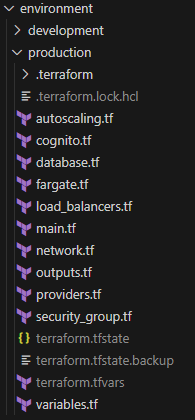
\includegraphics[height=0.4\pdfpageheight]{images/aws-repo-structure.png}
            \caption{Struktura plików Terraform}
            \label{fig:aws-repo-structure}
        \end{figure}

        Pliki \texttt{.tf} zawierają opis zasobów wdrażanych na serwery. Plik \texttt{.tfstate} przechowuje dokładny spis zasobów już wdrożonych wraz z ich unikalnymi identyfikatorami, sekretami, itd. Opis pozostałych plików:
        \begin{itemize}
            \item \texttt{main.tf} - wersje oprogramowania wykorzystywane w projekcie
            \item \texttt{providers.tf} - konfiguracja dostawcy AWS
            \item \texttt{variables.tf} - spis wszystkich zmiennych wraz z ich opisami i niektórymi wartościami domyślnymi
            \item \texttt{terraform.tfvars} - niewersjonowany plik zawierający wartości niektórych zmiennych; przede wszystkim przechowuje sekrety
            \item \texttt{outputs.tf} - zbiór przydatnych wartości wyjściowych, np. nazwa DNS Application Load Balancera
            \item \texttt{network.tf} - zasoby sieciowe: VPC, brama sieciowa, tablice routingu, podsieci
            \item \texttt{security\_groups.tf} - grupy bezpieczeństwa (działają jak zapora ogniowa - ang. firewall) konfigurujące przychodzący i wychodzący ruch sieciowy
            \item \texttt{cognito.tf} - dostawca tożsamości Amazon Cognito i jego konfiguracja
            \item \texttt{load\_balancers.tf} - Application Load Balancer, zasoby nasłuchujące na portach 80, 443 i 8080 oraz grupy celów
            \item \texttt{fargate.tf} - definicje zadań wykonywanych przy pomocy AWS Fargate oraz serwisy które nimi zarządzają
            \item \texttt{autoscaling.tf} - zestaw reguł pozwalających na automatyczne zmniejszanie lub zwiększanie liczby działających instancji modułów (frontendu i backendu)
            \item \texttt{database.tf} - konfiguracja bazy danych RDS
        \end{itemize}
    \subsubsection{Wykorzystane zasoby}
        \paragraph{Amazon Virtual Private Cloud (VPC):}
        Amazon VPC pozwala na tworzenie izolowanej, logicznie odseparowanej sieci w chmurze AWS. Umożliwia pełną kontrolę nad konfiguracją sieci, w tym zakresami adresów IP, podsieciami, trasami, bramami i konfiguracją reguł zapory sieciowej.
        
        \paragraph{Amazon Cognito:}
        Amazon Cognito umożliwia zarządzanie tożsamościami i autoryzacją użytkowników w aplikacjach internetowych oraz mobilnych. Zapewnia obsługę logowania użytkowników, synchronizacji danych oraz integracji z dostawcami tożsamości.
        
        \paragraph{Amazon Relational Database Service (RDS):}
        Amazon RDS to zarządzana usługa baz danych, która umożliwia łatwe konfigurowanie, działanie i skalowanie relacyjnych baz danych. Obsługuje popularne silniki, takie jak MySQL, \textit{PostgreSQL}, MariaDB, Oracle oraz SQL Server.
        
        \paragraph{Amazon Application Load Balancer (ALB):}
        Amazon ALB to rodzaj load balancera, który automatycznie rozdziela ruch aplikacji na wiele celów, takich jak kontenery, instancje EC2 lub funkcje Lambda. Jest zoptymalizowany do obsługi ruchu HTTP/HTTPS oraz oferuje zaawansowane funkcje, takie jak routing oparte na zawartości czy target groups.
        
        \paragraph{Amazon Elastic Container Service (ECS):}
        Amazon ECS to zarządzana usługa orkiestracji kontenerów, która umożliwia uruchamianie, zatrzymywanie i zarządzanie kontenerami Docker na klastrach instancji EC2 lub w ramach AWS Fargate (serverless). Jest w pełni zintegrowana z innymi usługami AWS.
        
        \paragraph{Amazon Certificate Manager (ACM):}
        Amazon ACM umożliwia łatwe zarządzanie certyfikatami SSL/TLS. Automatyzuje procesy wydawania, odnawiania i wdrażania certyfikatów dla aplikacji działających w AWS, eliminując potrzebę ręcznej konfiguracji.
        
        \paragraph{Amazon CloudWatch:}
        Amazon CloudWatch to usługa monitorowania zasobów i aplikacji AWS. Umożliwia zbieranie, przeglądanie i analizowanie metryk, logów oraz ustawianie alarmów. Zapewnia również możliwość automatycznej reakcji na zmiany wydajności systemu.
        
        \paragraph{Amazon Simple Storage Service (S3):}
        Amazon S3 to skalowalna usługa magazynowania obiektów, która pozwala na przechowywanie dowolnej ilości danych. Jest idealna do tworzenia kopii zapasowych, archiwizacji, hostowania zasobów statycznych i integrowania z aplikacjami chmurowymi.
        
        \paragraph{AWS Auto Scaling:}
        AWS Auto Scaling automatycznie dostosowuje liczbę zasobów obliczeniowych (np. kontenerów Fargate) w odpowiedzi na zmieniające się obciążenie. Zapewnia elastyczność, wysoką dostępność i optymalizację kosztów poprzez skalowanie w górę lub w dół w oparciu o zdefiniowane zasady.
    

\end{document}